\chapter[Spécifications fonctionnelles et techniques]{Les spécifications fonctionnelles et techniques}\label{ch:specifications-fonctionnelles-techniques}

J'ai travaillé sur le projet Pipeline documentaire sous la direction de ma tutrice au sein de l'équipe de développement de SuiviDeFlotte. Avant de commencer, étant donné la complexité du projet, nous avons tenu plusieurs réunions avec le propriétaire du produit. Celui-ci nous a expliqué en détail ses idées concernant le projet, et bien sûr, nous avons également partagé nos réflexions.

Dans le chapitre précédent, je crois que c'était évident que notre propriétaire de produit avait une vision précise de la manière dont l'application devait être construite et de son fonctionnement. Par conséquent, nous n'avons pas eu besoin de débuter par l'analyse d'un cahier des charges pour identifier les entités et les relations qu'il pourrait contenir. Cette étape avait déjà été accomplie.

Il a également été convenu que nous développerions ce projet en utilisant le framework Laravel et que nous le déploierions dans des conteneurs Docker. Nous avons constaté que le framework Laravel offrait tous les éléments nécessaires pour ce projet : commandes, gestion des événements, mise en file d'attente des tâches, ainsi que des fonctionnalités pour créer facilement une API, entre autres. De ce fait, ce choix nous est apparu comme judicieux, d'autant plus qu'il avait déjà été utilisé pour de nombreux autres projets au sein de la société, ce qui signifiait que les développeurs possédaient une solide expérience avec cet outil.

L'utilisation de conteneurs Docker pour le développement n'était pas encore une pratique courante au sein de l'entreprise. Cependant, une transition était prévue pour que tous les projets soient conteneurisés. Par conséquent, lors du lancement de nouveaux projets, leur conteneurisation était envisagée dès le début.

Au cours de ces réunions, de plus en plus de détails ont été précisés et nous étions prêts à entamer le projet. Néanmoins, il restait encore un travail de conception à accomplir pour définir en détail l'implémentation de ce projet dans ces cadres.

Le plan de mise en œuvre du projet dans le système de contrôleurs, de commandes et d'événements de Laravel est présenté dans le diagramme d'activités de la Figure~\ref{fig:import-activity-diagram}. Comme le montre le diagramme, la réalisation du projet dans Laravel nécessite un élément qui n'est présent qu'implicitement dans le schéma architectural, à savoir l'écouteur d'événements entre les déclencheurs et la file d'attente.

\begin{sidewaysfigure}
    \centering
    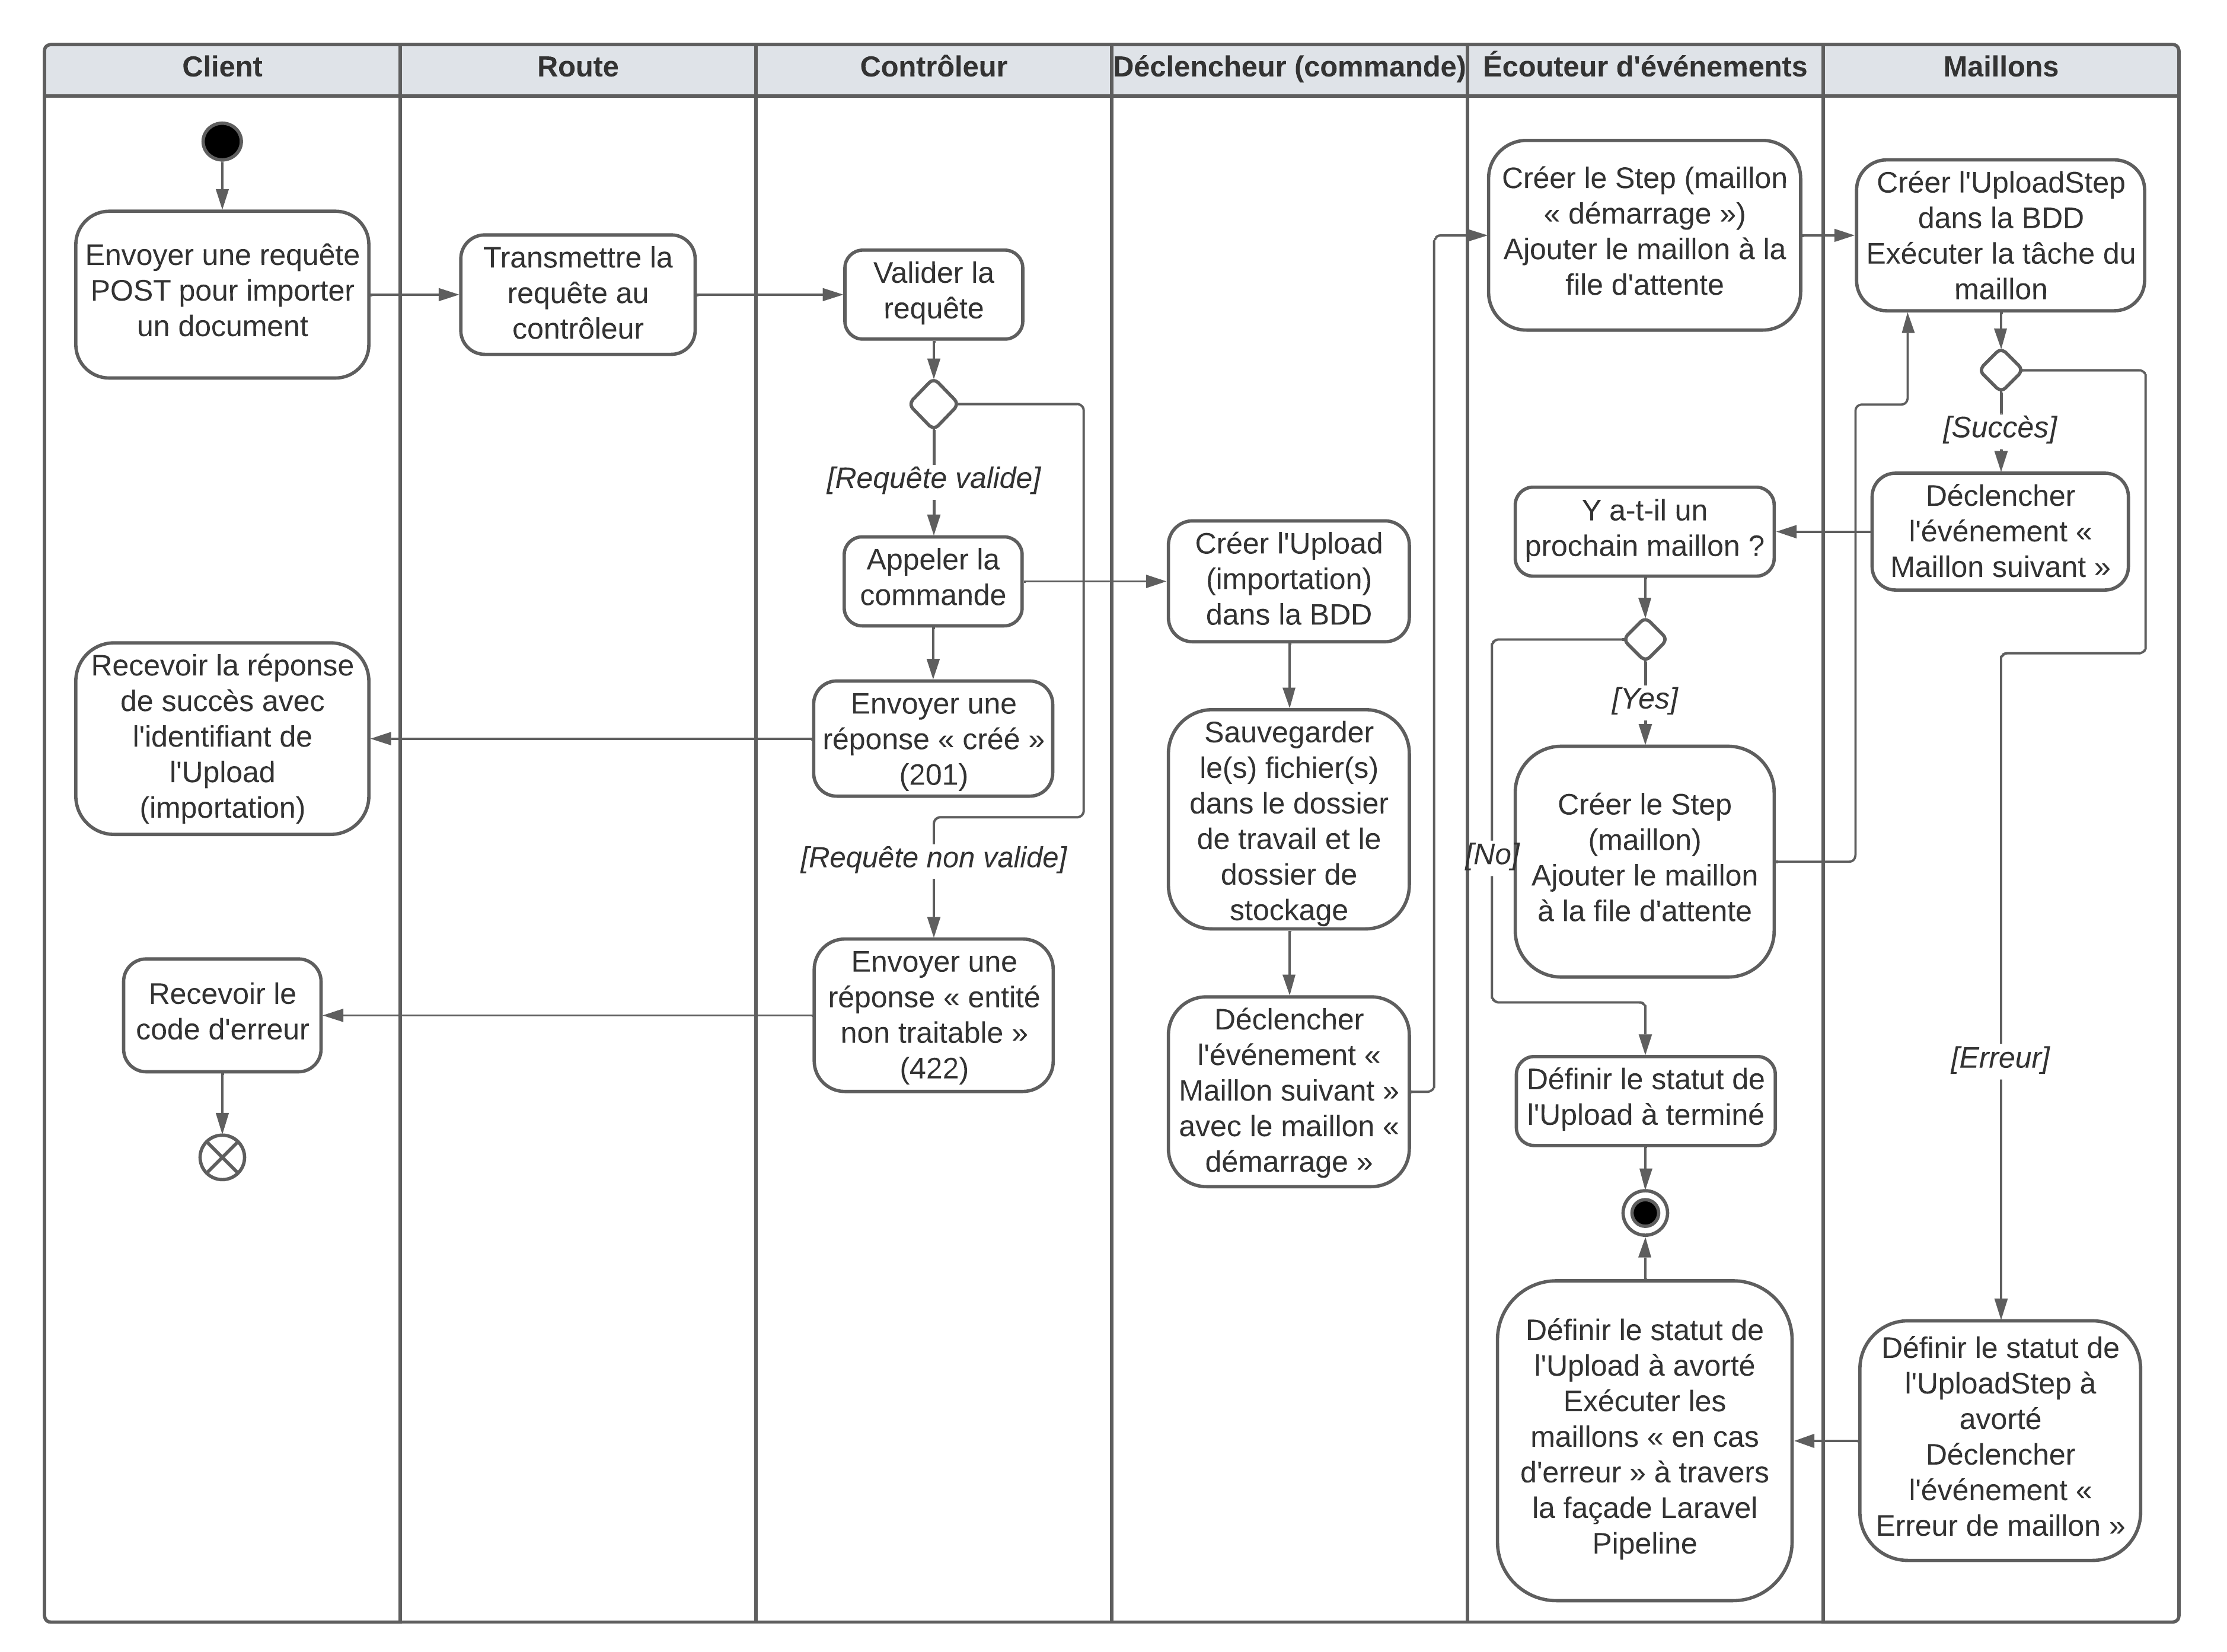
\includegraphics[width=\textwidth]{img/import-activity-diagram}
    \caption{Diagramme d'activité de l'envoi d'une requête POST pour importer un document.}
    \label{fig:import-activity-diagram}
\end{sidewaysfigure}

Le diagramme de classes permet d'obtenir une vue plus détaillée du fonctionnement du projet (Figure~\ref{fig:class-diagram}). Le même processus que celui illustré dans le diagramme architectural et le diagramme d'activité peut être suivi ici également, en commençant par les déclencheurs (la classe abstraite \emph{\Verb|UploadTrigger|} et ses classes enfants). Au début du processus d'importation, ces classes instancient un modèle \Verb|Upload|, l'enregistrent dans la base de données et lancent l'événement \Verb|NextStepEvent|. L'écouteur d'événements (classe \Verb|StepEventSubscriber|) est à l'écoute de cet événement et instancie l'une des classes enfants de la classe abstraite \emph{\Verb|Step|} (maillon) en fonction de la configuration du type de fichier importé qui lui est fournie par la classe \Verb|UploadType|. Le maillon instancie un modèle \Verb|UploadStep|, l'enregistre dans la base de données, exécute sa propre tâche et lance à nouveau un événement \Verb|NextStepEvent| ou, en cas d'erreur, lance l'événement \Verb|StepErrorEvent|. Ensuite, le cycle recommence avec l'écouteur d'événements, lequel consulte le fichier de configuration à l'aide de la classe \Verb|UploadType| pour trouver le maillon suivant, s'il en existe un. Dans certains cas, par exemple, lorsqu'un fichier fait l'objet d'une reconnaissance optique de caractères (OCR), les résultats sont enregistrés dans la base de données à l'aide du modèle \Verb|UploadResult|. C'est la tâche du maillon \Verb|PersistResult|. Le modèle physique des données, qui comprend les tables de base de données correspondantes aux modèles \Verb|Upload|, \Verb|UploadStep| et \Verb|UploadResult|, est illustré à la Figure~\ref{fig:pmd}.

\begin{figure}[ht]
    \centering
    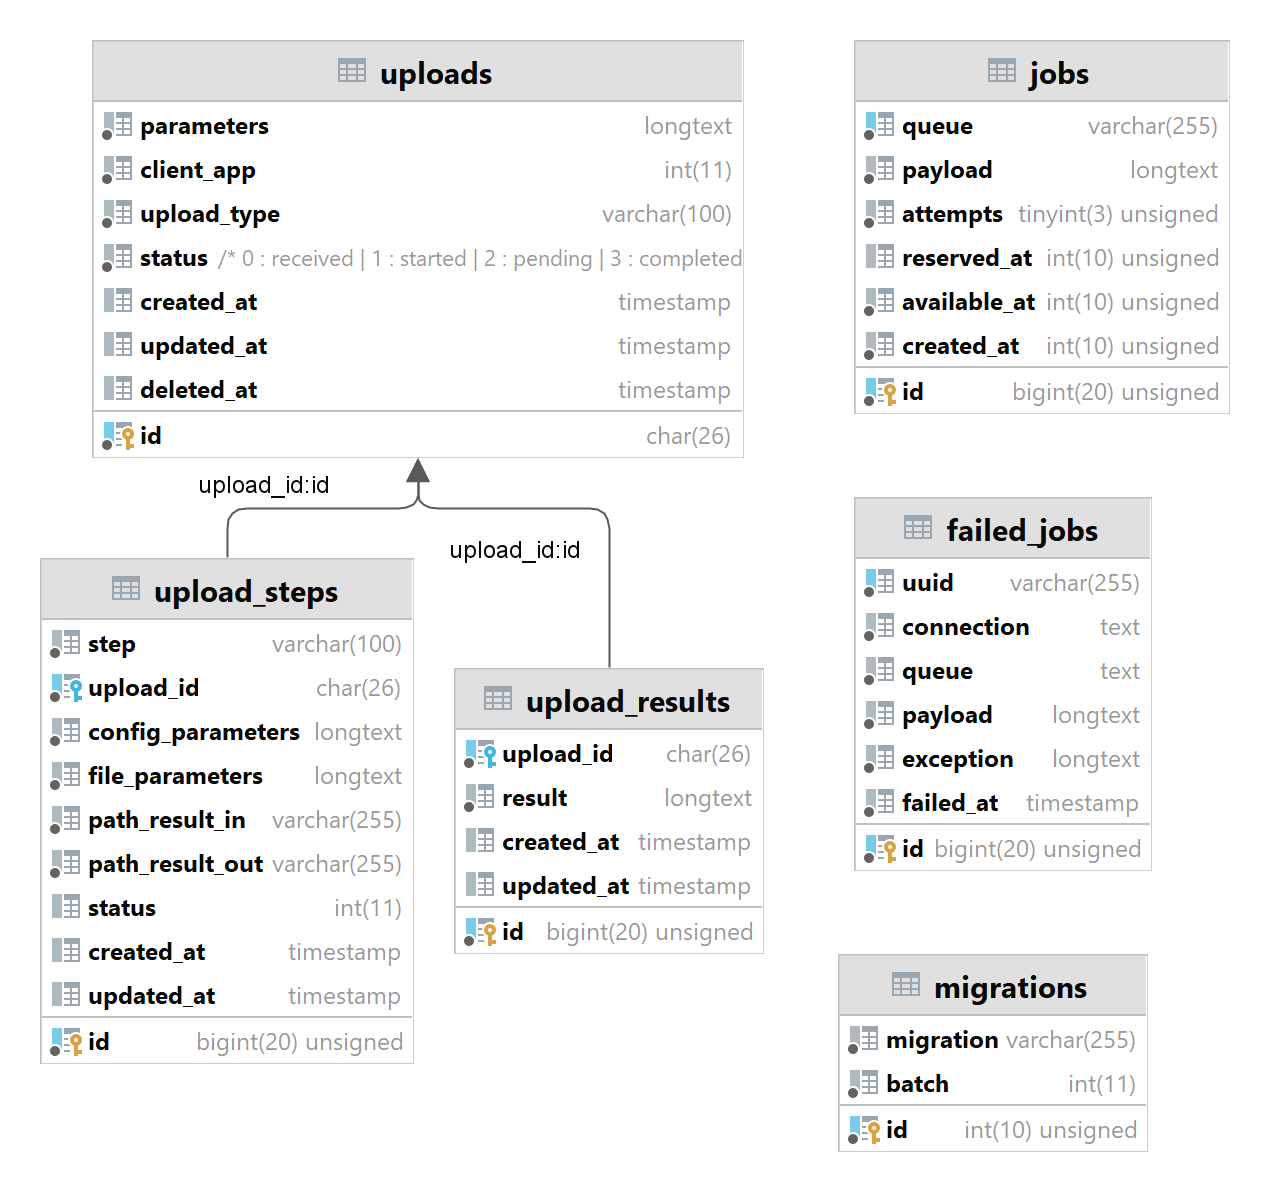
\includegraphics[width=\textwidth]{img/sdf_db}
    \caption{Modèle physique des données du Pipeline documentaire.}
    \label{fig:pmd}
\end{figure}

\begin{sidewaysfigure}
    \centering
    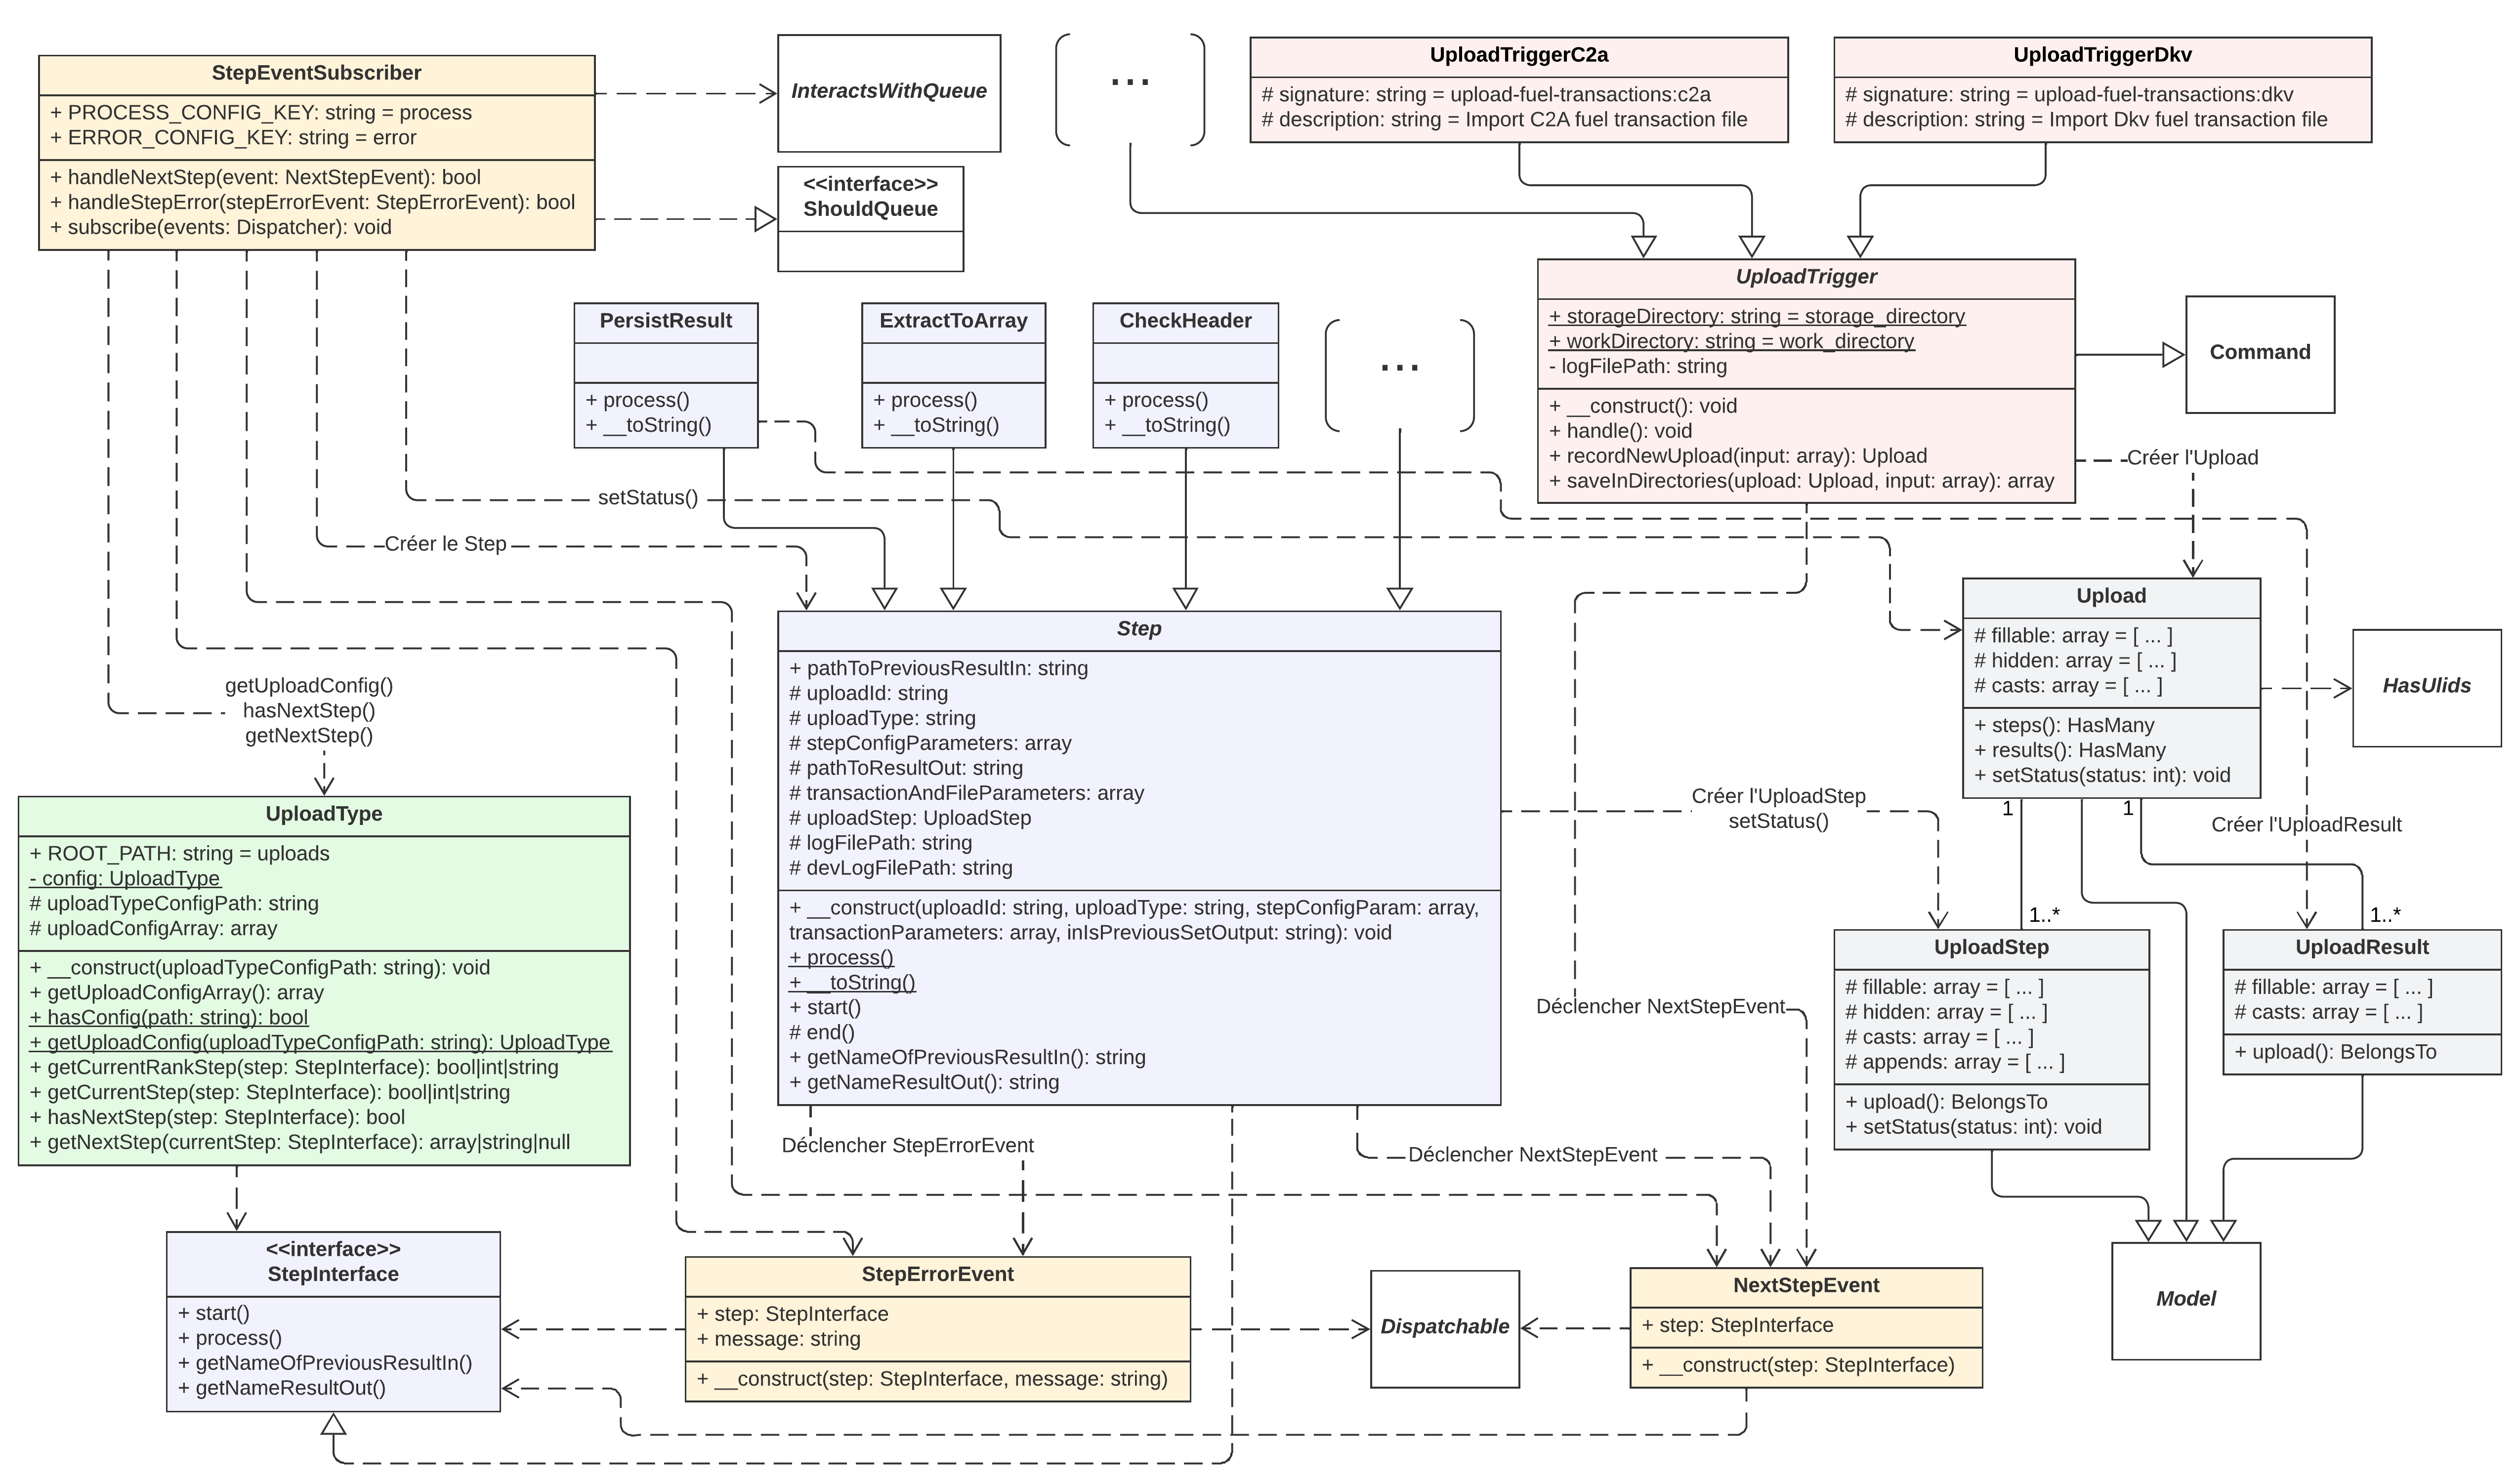
\includegraphics[width=\textwidth]{img/class-diagram-2}
    \caption{Diagramme des classes principales du Pipeline documentaire.}
    \label{fig:class-diagram}
\end{sidewaysfigure}